\documentclass[8pt,a4paper]{extarticle}
\usepackage{graphicx}
\usepackage{lscape}
\usepackage[margin=0.5cm, landscape]{geometry}
\usepackage{multicol}
\usepackage{amsmath}



\begin{document}
\thispagestyle{empty}
\noindent
  \textbf{Architetture ICT complesse (Information and Comunication Technology) 2019/2020 ©}
\begin{multicols*}{4} \setlength{\columnseprule}{0.4pt}
	 \section{Storage architectures, technologies and systems}
	    \subsection{Evoluzione}
	    \subsubsection{Fattori legati al Business}
		I dati sono sono importanti per le aziende moderne e bisogna proteggerli per non perderli e garantire sempre il loro accesso. Bisogna gestire le situazioni critiche mettendo i dati in un posto sicuro, garantendo la continuità al business. I costi per la manutenzione degli storage sono maggiori degli acquisti e c'é bisogno di semplificare l'architettura.
\\Le infrastrutture devono essere: \textbf{efficienti}, \textbf{affidabili}, \textbf{scalabili}, \textbf{gestibile}, \textbf{basate su standard} e \textbf{ragionevolmente economico}.
		\subsubsection{Fattori tecnici}
		Le ultime tecnologie sviluppate hanno permesso di sviluppare nuove applicazioni (internet, multimedia, BI, ...). Di conseguenza c'é stata una maggiore richiesta di: \textbf{capacità d'archiviazione, performance, affidabilità}.
		\subsubsection{Insidie degli approci tradizionali}
		Alla fine del '97 la velocità del network supera quello dello storage. Gli approci tradizionali hanno diversi svantaggi quali: "\textbf{attaccati direttamente al server, bus parallelo SCSI usato come interconessione,  accessi diretti al server, se il server è inattivo l'archiviazione non è accessibile, numero di dischi per controller è limitato in un server, ...}. Questo approcio non è una buona architettura per la scalabilità! 
		\subsubsection{Cambio di paradigma}
		Per risolvere il problema delle reti veloci che mettono sotto pressione i server, che generano un overload delle richieste, si è dovuto cambiare dallo \textbf{storage collegato direttamente a quello condiviso}, con il seguente schema:
		\begin{itemize}
			\item L'archiviazione può essere accessibile da più server
			\item Il carico di lavoro può essere distribuito su più server
			\item Gli storage possono essere spostati spostati da un server all'altro
			\item Gestione centralizzata dello storage aziendale 
		\end{itemize}
		
		\subsubsection{Crescita dei dati}
		Con la nascita degli IoT la quantità di dati sono esplosi, proprio perché lavorano 24/24, rispetto all'interazione dell'uomo con il device (videocamere, sensori, ecc...). Questa crescita ha umentato drasticamente i costi del IT con: più capacità di storage (e costi), grandi backup, ecc... \\ ILM (Information Lifecycle Management) permette le strategie per l'amministrazione di sistemi di archiviazione su dispositivi informatici.
		\subsubsection{Aspetti legali}
	 	Regole nazionali e internazionali impongono alle aziende delle regole per l'archiviazione, la conservazione e la sicurezza dei dati. La conformità è quindi un problema che influisce sul ICT e ILM è un modo per supportarla.
	 	
	 	\subsection{Storage}
	 	Uno storage system è una tecnologia designata e usata per la conservazione dei dati digitali. Ci sono 4 gerarchie di storage systems:
	 	\begin{itemize}
	 		\item \textbf{Primario} - Accesso diretto dalla CPU (RAM, ROM, cache)
	 		\item \textbf{Secondario} - Non diretto dalla CPU (HDD, SSD)
	 		\item \textbf{Terziario} (nearline) - Uso di robot per caricare/scaricare in un drive
	 		\item \textbf{Off-line} - Supporti d'archiviazione mantenuti offline e richiede l'intervento umano per caricare/scaricare in un drive
	 	\end{itemize}
	 	Parametri per la differenziazione dei livelli di gerarchia: performance, mutability, latency, addressability, capacity, security, energy use, cost per capacity.
	 	\subsubsection{Tipi di storage}
	 		\begin{itemize}
	 			\item \textbf{Blocchi} - Su dichi e memorie (tracce e settori)
	 			\item \textbf{File} - Cartella in ordine logico fisso (file path, file name, Date)
	 			\item \textbf{Oggetti}  - Container di dimensione flessibile (UID, Data e metadati)
	 		\end{itemize}
	 		\subsubsection{Storage a blocchi}
	 		I dati sono salvati in blocchi di dimensione fissa, senza nessun metadato di alto livello. Accessibile da OS con un "mount" e tramite un file system si decide come i blocchi sono accessibili, combinati e modificabili. L'applicazione scrive sui data block, ideale per l'archiviazione primaria ad alte prestazioni. Casi d'uso: strutture DB, volumi virtuali, Workloads, High change content, Random R/W e Bursty I/O.\\
	 		\textbf{Accesso ai dati:} Applicazione scrive blocchi $\to$ Inietor SW/HW $\to$ Controller $\to$ dati scritti sul device come data block.

	 		\subsubsection{File storage}
	 		I file sono accessibili in modo casuale, chiamati con operazioni IO attraverso un manipolatore, vengono organizzati in directory (file strutturati) e possono avere diversi livelli (anche combinati): \textbf{file system logici, virtuali, fisici e accesso di rete}. Hanno supporto POSIX e possono essere trattati attraverso dati non strutturati (stream o oggetti), dati strutturati e blocchi.
	 		
	 		\subsubsection{Storage ad oggetti}
	 		Contiene tipicamente le reposity, URL, metadati, ObjectID e versioni. I casi d'uso sono: \textbf{per i cloud pubblici/privati/ibirdi, archiviazione, archiviazione senza server, IoT, machine learning,  ecc...}. Non richiede un "mount" per accedere ai dati e sono accessibili da qualsiasi endpoint.
		\subsection{Confronto e tendenze della tecnologia del disco}
		Le interconnessioni parallele, come: \textbf{ATA e SCSI}, sono state sostituite con quelle seriali (\textbf{SATA, SAS, NL-SAS e Fibrechannel}), perché avevano problemi di: overhead, inclinazione del segnale, crosstalk (un segnale che si imprime sul filo affianco), riflessione di cavi e connettori, ecc. Con l'interconessione seriale si hanno vantaggi quali: \textbf{velocità, affidabilità e scalabilità}
		
		\subsubsection{HDD}
		Le tecnologie attuali per per questa tipologia di dischi sono: \textbf{ATA/SATA} (desktop), \textbf{SAS / NL-SAS / Fibrechannel} (servers) e \textbf{SCSI} (legacy). Le differenze tra una tecnologia e l'altra sono: \textbf{prezzo, performance, affidabilità e scalabilità}. \\ Questa tecnologia ha un collo di bottiglia con le operazioni I/O, dove la maggior parte del tempo viene spesa per cercare, leggere e scrivere i dati. Per le operazioni R/W le IOPS scendono a \textbf{livelli insostenibili con sistemi multicore, ambienti virtualizzati e applicazioni con un flusso intensivo di dati}.
		\begin{itemize}
			\item \textbf{SATA}:  Hanno una rotazione tra i 5.4K e 7.2K, sono molto convenienti e vengono utilizzate più per le grandi capacità piuttosto che per le performance.
			\item \textbf{SAS} (Serial-Attacched SCSI): È uno standard che, preservando il SW SCSI, viene spostato dall'interfaccia parallela all'interconessione seriale e ha un ampio intervallo di indirizzi. Puo usare cavi superiori i 10Km e ha un data rate di 12 Gbit/s. Può avere connessioni simultanee attive ed è molto più affidabile rispetto al SATA grazie ad BER (Bit Error Rate) molto basso. Per uso aziendale. 
			\item \textbf{NL-SAS} (Nearline-SAS): Sono degli HDD SATA con l'interfaccia SAS, dove possono sfruttare le funzionalità aziendali su uno SATA, quali: queuing, data channels concorrenti e supporto di più host. Non hanno le performance di un SAS, ma abbattono i costi per avere molto più spazio in un infrastruttura SAS.
		\end{itemize}
		
		\subsubsection{SSD}
		Tecnologia inizialmente costosa (rispetto al HDD) usata in ambito militare e scientifico, viene usato per accessibilità ai dati ad alte prestazioni ma \textbf{non per archiviazione dati}. SSD sono ottime soluzioni per le applicazioni con molte letture e poche scritture ai dati (Es. web server). Memorizza elettronicamente i dati e non garantisce una lunga persistenza nel tempo e usa un'interfaccia elettronica compatibile con quella tradizionale a blocchi. Ha molti vantaggi quali: \textbf{resistenza agli urti, basso cosumo elettrico, silenziosità e bassa latenza e tempo d'accesso (performance)}. È composto da un controller (processore incorporato che esegue codice a livello firmware), delle memorie NAND e cache. È disponibile il protocollo NVMe che ne implementa il parallelismo rispetto all'attacco "tradizionale" SATA e ci sono 4 tecnologie per la scrittura sulle celle di memoria:
		\begin{itemize}
			\item \textbf{SLC} (single-level cell): Viene salvato 1 bit per ogni cella, è molto veloce in R/W, migliore durata, è la \textbf{NAND più costosa sul mercato} e le capacità sono ridotte. Uso: \textbf{industriale / aziendale}
			
			\item \textbf{MLC} (multi-level cell): 2 bit per ogni cella, meno affidabile e durevole di un SLC, minor costo e maggiore capacità. Uso: \textbf{Consumer / Gamer}
			
			\item \textbf{TLC} (triple-level cell): 3 bit per ogni cella, usato solo per lato consumer, R/W e vita dell'hardware molto più bassa le precedenti. Uso: \textbf{Consumer}
			
			\item \textbf{QLC} (quad-level cell):4 bit per cella, più capacità e basso costo dell'HW. Performance e vita equivalgono quasi al TLC. Uso: \textbf{Utenti con grande richiesta di archiviazione dati}
		\end{itemize}
Il controller, cuore della performance sugli SSD, ha come funzione quello di: \textbf{correggere gli errori, Wear leveling} (distribuire i dati su più celle invce che la stessa)\textbf{, mappare i blocchi danneggiati, scrubbing e management in lettura, R/W caching, garbage collector ed encryption}. 
\\ \\
\textbf{NVMe e NVMe-oF:} è un protocollo di archiviazione creato per accelerare il trasferimento di dati tra sistemi e unità a stato solido su un bus PCIe. NVMe-oF (over Fabbric) è un protocollo di trasporto su rete per connettere dispositivi remoti a livello di blocchi. Esistono pochi tipi di NVMe-oF a dipendenza del protocollo di trasporto (es: Fibrechannel $\to$ \textbf{NVMe-FC}).

\subsection{Disk Subsystems}
\subsubsection{JBOD - Just a Bunch of Disks}
Soluzione economica rispetto ad un RAID, dove ogni file da archiviare è salvato all’interno di un unico disco, ma con la conseguenza che se uno si rompe i dati sono persi. Questi hard disks vengono collegati ad un server, che si occupa di gestirli e connetterli attraverso un SW dove usa tutte le sue risorse. 
\begin{center}
    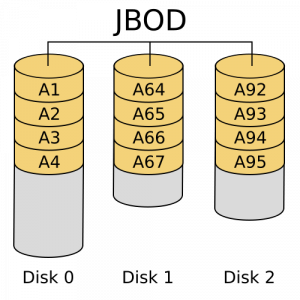
\includegraphics[width=.4\linewidth]{src/JBOD.png}
  \end{center}

\subsubsection{Intelligent Disk Subsystems}
Non sono solo semplici contenitori di dischi, ma ci sono controller che permettono di gestire i livelli RAID (prima era il server che se ne occupava. RAM interna al disk array utilizzata come cache, quindi come buffer per migliorare le prestazioni).
Ci sono differenti possibilità di canali di ridondanza I/O:\\
\textbf{Attivo-passivo}: Il canale secondario di I/O è usato solamente quando la primaria fallisce.\\
\textbf{Attivo-attivo (W/O balancing)}: I dischi sono raggruppati da 2 o più gruppi, dove vengono gestiti i canali sui cui devono operare. In caso di problemi su un canale, il traffico viene spostate su un altro.\\
\textbf{Attivo-attivo (load balancing)}: I canali sono attivi ed è il controller che bilancia il traffico I/O tra i due.
\subsubsection{RAID Technology}

\textbf{RAID 0 - Striping}: Divide il file in 2 parti uguali e le salva su due dischi differenti. Non c'é ridondanza e non garantisce il recupero dei dati in caso di danneggiamento del disco, ma in compenso si ha una R/W veloce dei dati.
		\begin{center}
    			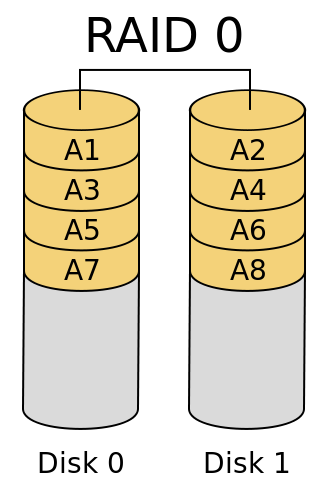
\includegraphics[width=.3\linewidth]{src/raid0.png}
  		\end{center}
\textbf{RAID 1 - Mirroring}: Crea due copie esatte dello stesso file e le salva in due dischi differenti. Sacrifica una grande quantità di spazio ma garantisce un elevato tasso di sicurezza contro la perdita di dati.
		\begin{center}
    			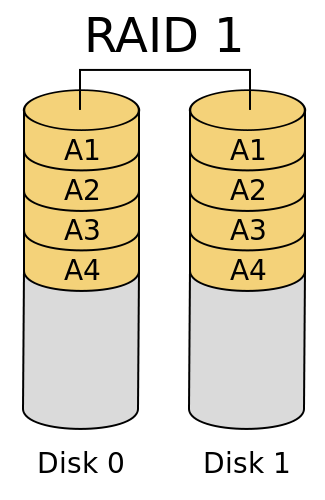
\includegraphics[width=.3\linewidth]{src/raid1.png}
  		\end{center}
\textbf{RAID 3  Byte-level striping}: Suddivide ogni file in byte e salva ciascuna parte in un disco differente creando una copia compressa nel disco di parità. Permette di accedere ad un solo file alla volta.
		\begin{center}
    			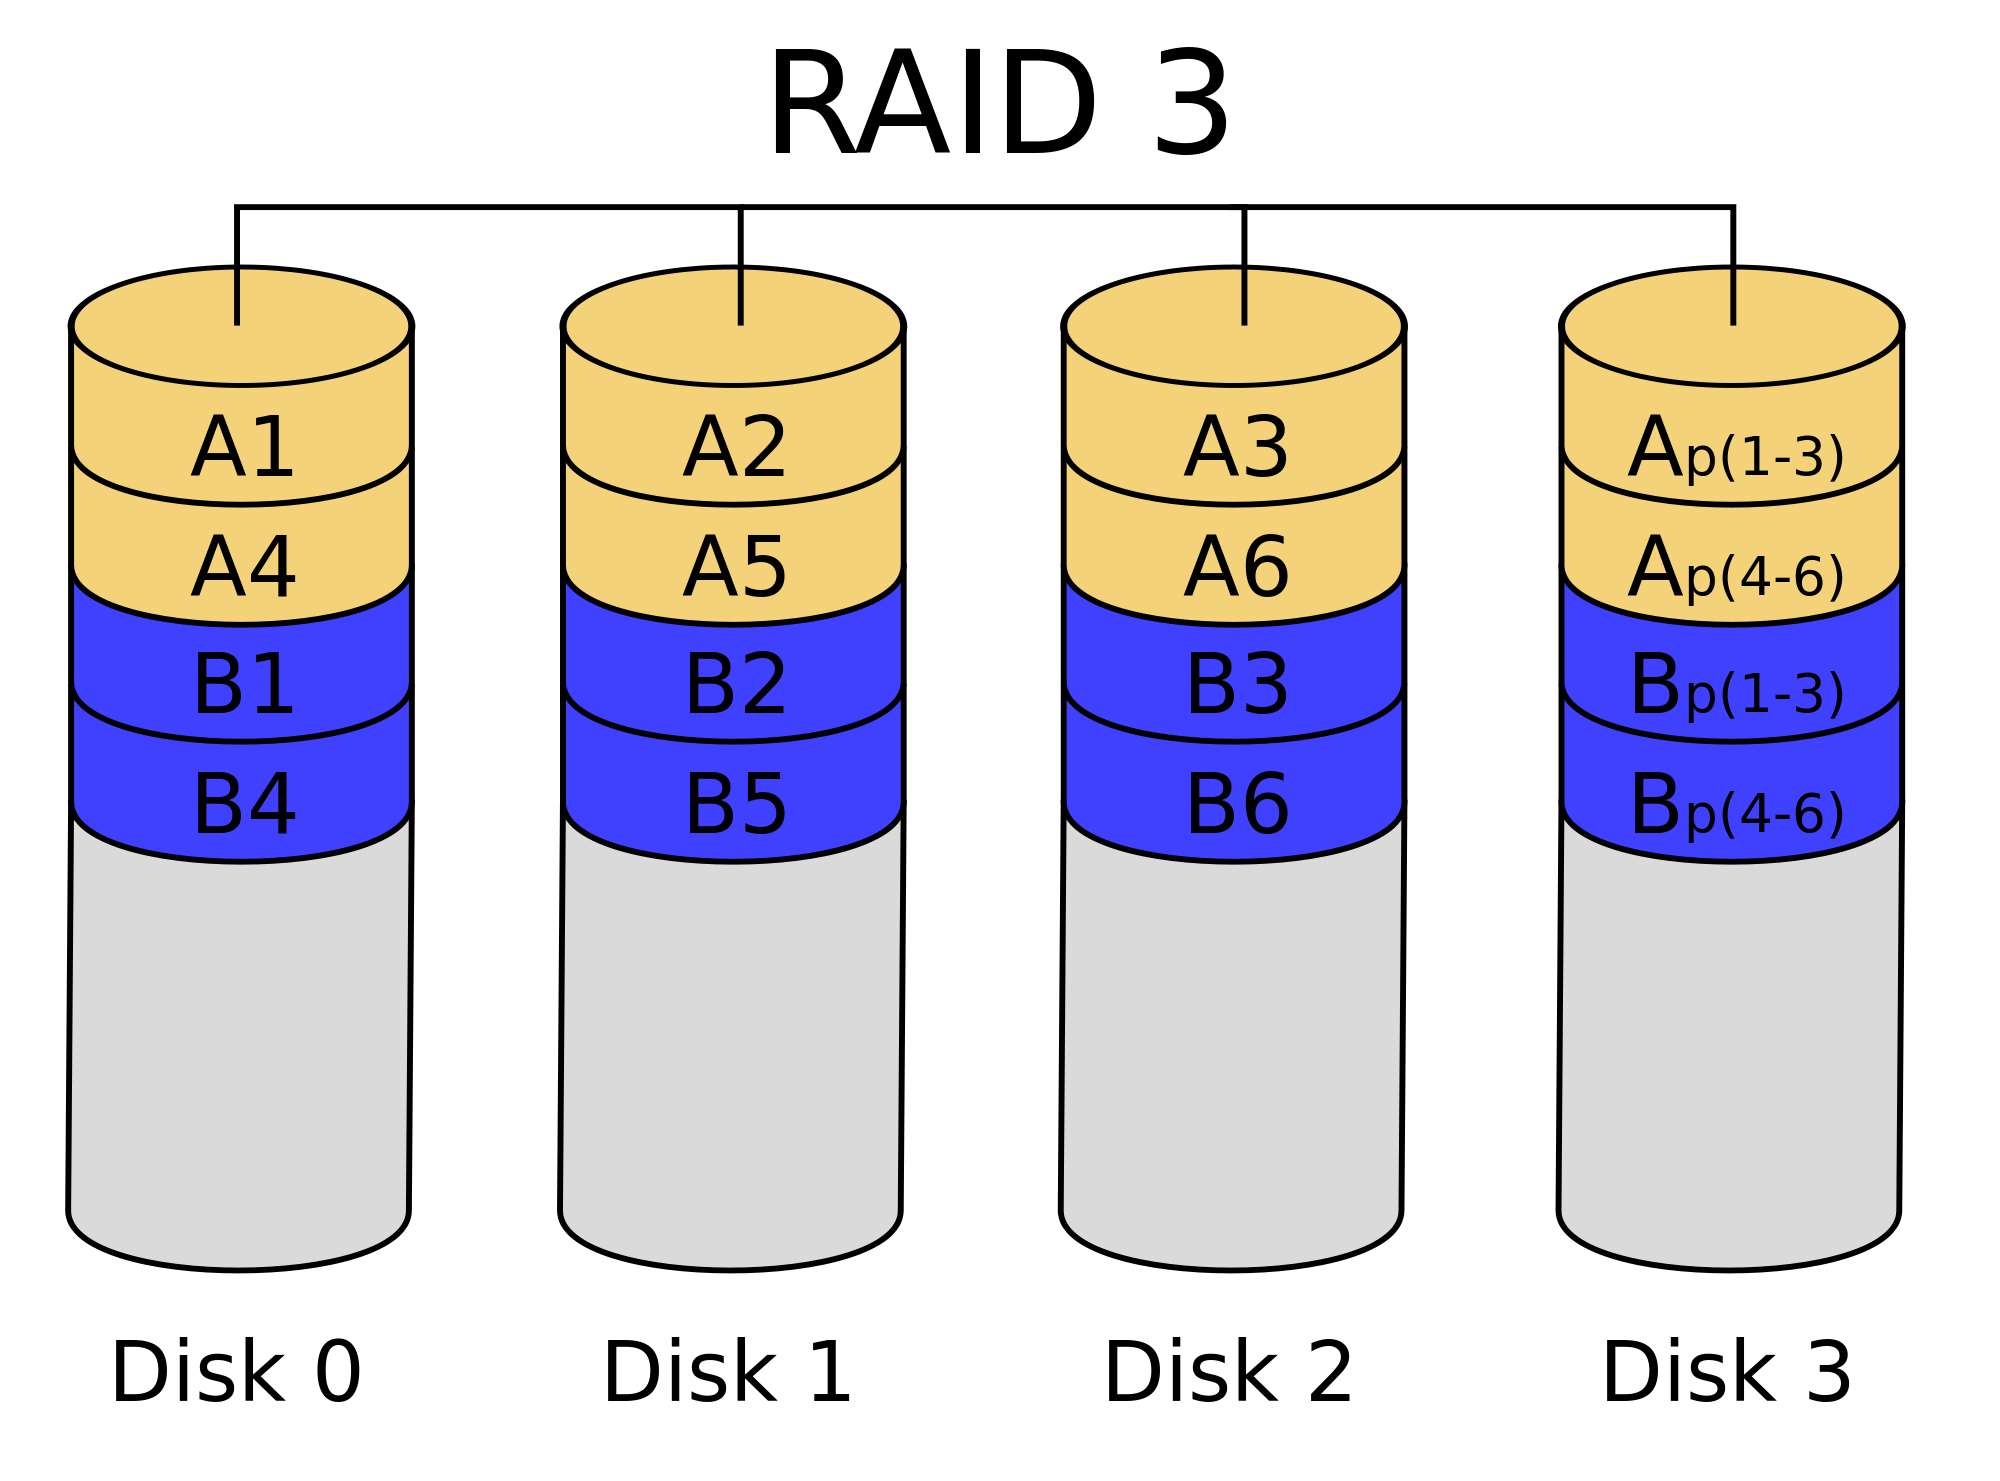
\includegraphics[width=.5\linewidth]{src/raid3.png}
  		\end{center}
\textbf{RAID 4 - Block-level striping}: Suddivide ogni file a livello di blocchi e salva ogni blocco in un disco differente creando una copia compressa nel disco di parità.
		\begin{center}
    			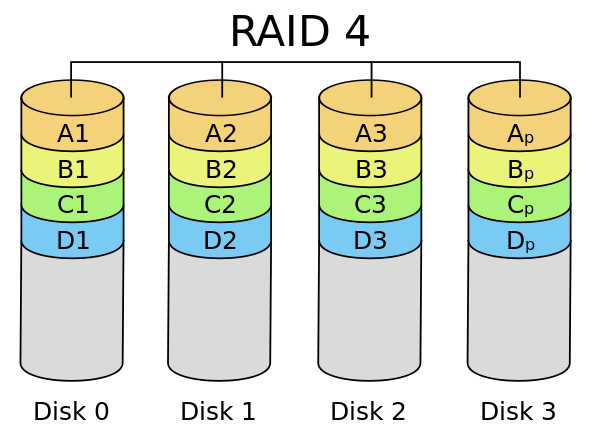
\includegraphics[width=.5\linewidth]{src/raid4.png}
  		\end{center}
\textbf{RAID 5 - Block-level striping con parità distribuita}: Suddivide i dati di parità di ciascun file in blocchi e salva ciascun blocco di dati su un disco diverso. Salva l’intero insieme dei dati di parità (non suddivisi in blocchi) di ciascun file in un ulteriore disco. Limita lo spazio necessario all’archiviazione e permette di accedere a più file contemporaneamente, dove se um disco è in uso, vengono fornite le informazioni dal disco di parità (R/W lento perche dei dati di parità sono compressi).
		\begin{center}
    			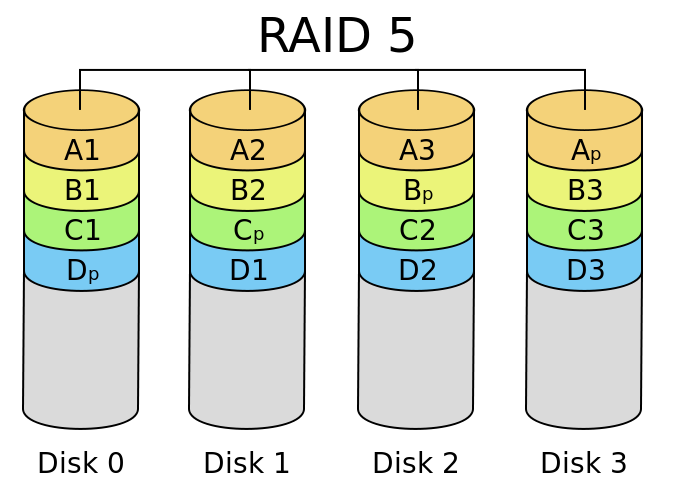
\includegraphics[width=.5\linewidth]{src/raid5.png}
  		\end{center}
\textbf{RAID 6 -  Block-level striping a doppia parità}: Suddivide il file in blocchi e salva ciascuno blocco in un disco diverso, creando e salvando 2 copie dei dati di parità di ogni file su un disco diverso. La lettura dei file è più veloce perché non è necessario recuperare dati compressi per rendere il file reperibili, ed in caso di guasto esistono ben due dischi che contengono le informazioni per recuperare i file.
		\begin{center}
    			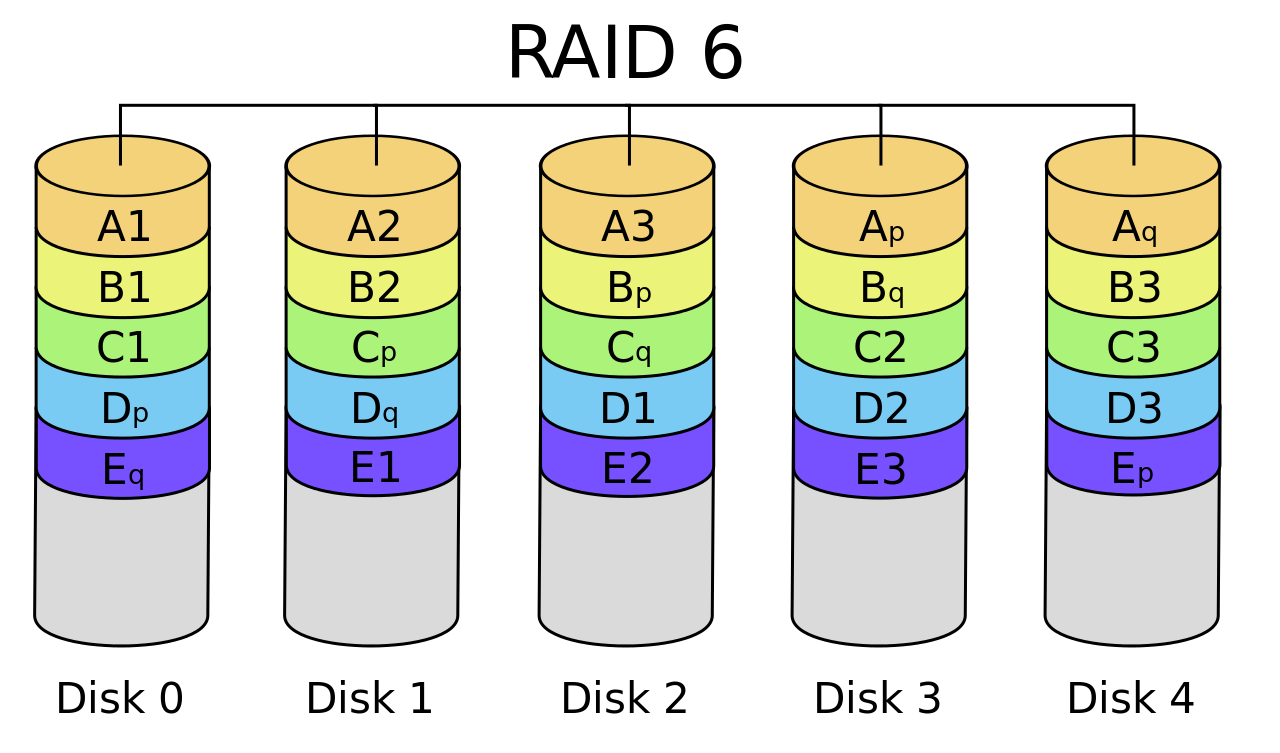
\includegraphics[width=.5\linewidth]{src/raid6.png}
  		\end{center}
\textbf{RAID 10 - Stripe of mirrors}:
			\begin{center}
    			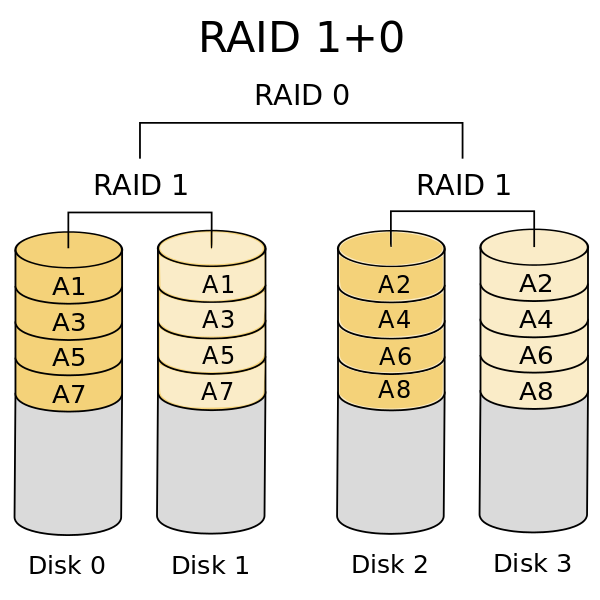
\includegraphics[width=.5\linewidth]{src/raid10.png}
  		\end{center}
\subsubsection{Volume Management}
Il disk subsystems è equipaggiato con un software interno per la gestione dei volumi. Previene di sprecare le risorse e supporta RAID multipli a vari livelli e varie funzioni alle VM. Tutti i dischi fisici sono incapsulati all'interno, dove è possibile successivamente creare delle unità logiche.

\subsubsection{Thin Provisioning}
È una metodologia di come utilizzare la tecnologia di virtualizzazione per avere più risorse fisiche di quanto non sia in realtà a disposizione, per ogni host. L'ambiente di storage è condiviso e permette di ottimizzare l'utilizzo delle risorse. Questa metodologia elimina quasi tutti i whitespaces e aumenta le prestazioni di utilizzo del 10%. 

\subsubsection{LUN masking (Logical Unit Number)}
È un processo di autorizzazione che rende un numero di unità logica disponibile per alcuni host e non disponibile per altri host. Ogni volume è identificato con un \textbf{ID LUN} e può essere assegnato a uno o più host.

\subsubsection{Snapshots / Istant Copies}
Memorizza quali blocchi fanno parte di un certo volume in quel momento, non copia i blocchi subito. Quando poi i blocchi vengono modificati, allora il sistema effettua un copia del blocco prima che venga modificato. Permette un backup consistente, è una struttura che consente l'accesso ad una versione vecchia dei dati, al momento in cui è stato fatto lo snapshot. Contiene solo la copia dei blocchi che sono stati cambiati. Come ci si assicura che al momento dello snapshot il volume è consistente? Dal livello alto, dall'applicazione, parte la richiesta di
snapshot. Un disk array non può sapere quando il volume è consistente poichè vede solo blocchi.

\subsubsection{Business Continuance Volume}
È il termine per una copia indirizzabile in modo indipendente di un volume di dati, che utilizza una tecnica di mirroring avanzata per scopi di continuità aziendale. La copia può essere usata per qualsiasi scopo come backup, ecc.. \\ La copia viene scollegata, per un certo lasso di tempo, dov'é temporaneamente congelata. Il sistema funziona come RAID 0, e questa copia può essere utilizzata per altre operazioni e gli aggiornamenti vengono eseguite sul volume di produzione.

\subsubsection{Replication}
Il contenuto di un volume può essere clonato su un'unità remota senza l'intervento del sistema host. I 2 subsystem devono essere connessi e configurati per la replicazione, dove può essere sincrona o asincrona.
\begin{center}
    			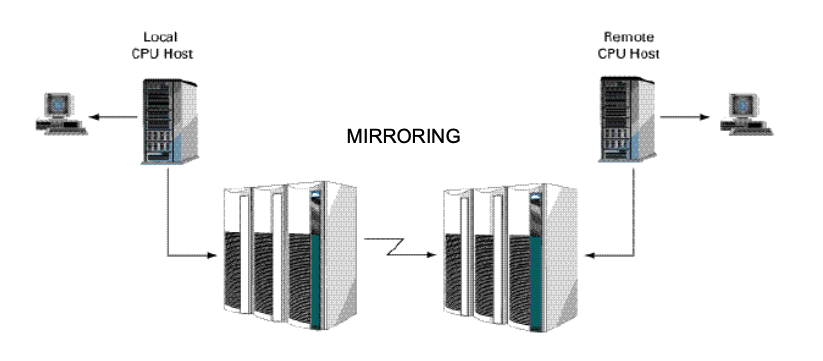
\includegraphics[width=.8\linewidth]{src/replication.png}
  		\end{center}
  		
\subsubsection{Array with flash cache}
È possibile aumentare le prestazioni con svariate tecniche con l'utilizzo di cache. A dipendenza della tecnica utilizzata, per esempio DRAM, si ha una diminuzione di latenza sul I/O di quasi 10 volte, ma richiede SSD di tipo SLC, perciò molto più cari. Richiede un UPS o un sistema di diagnostica interna per garantire la persistenza dei dati in caso di mancanza di corrente.

\subsubsection{Object-Based Storage}
Utilizzato soprattutto nel cloud, poiché permette di definire oggetti e questo facilità l’utilizzo alle applicazioni. Caratterizzati da dati non strutturati dati embedded e dati immutable, Dati di cui non si conosce la posizione e nessuna gestione dei Volume. Scalabilità, sicurezza, durabilità, consistenza e cross-platform. Si concentra sulla gestione dei dati per tipo a discapito della loro posizione. Sono visualizzati come unico spazio, indipendente dai nodi, garantisce eventual-consistency (garantita consistenza finale) e permette policy più sofisticate es: dati nuovi su tutti i dischi, dati di 3 anni in archivio e quelli di 10 vengono cancellati. \\
L'oggetto contiene dati, metadati e un UID indicizzato.

\subsubsection{Software aggiuntivo}
Sebbene queste tecnologie sono trasparenti, è possibile utilizzando software aggiuntivo avere funzioni più avanzate come: backup più veloce e consistente, deduplicazione, spindown, disaster recovery, remote mirroring e configurazioni più flessibili (data tiering).
\end{multicols*}
\end{document}

